\subsection{\href{http://www.softron.biz/}{Softron}}
   \hypertarget{subsec:softron}
   La empresa Softron S.A provee soluciones al mercado mayorista de proveedores de energia, instalando medidores de consumo y ofreciendo el servicio de monitore remoto. \\
   Para dicha emprea se desarrollaron placas de integracion entre SBC, computadoras en una placa, y perifericos como, salidas de rele, entradas IO's, fuentes de alimentacion, soporte para modulo GSM y dual SIM, entre otras opciones. Se pueden ver algnas fotos de la placa desarrollada en la figura \ref{fig:softron1} para la cual se realizaron varios prototipos y se genero toda la documentacion de fabricacion en volumen. \\
   Por otra parte tambien se disenaron dispositivos inalambricos para monitoreo de temperatura usando redes Zigbee en modo mesh, se pueden ver algunas fotos de los equipos fabricados en la figura \ref{fig:softron}. \\
   \begin{figure}
      \begin{center}
         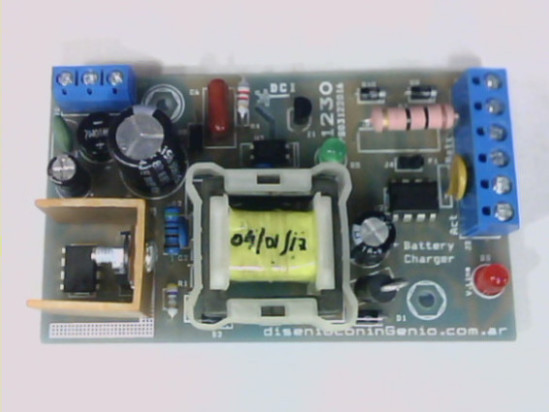
\includegraphics[width=0.24\textwidth]{softron1.jpg}
         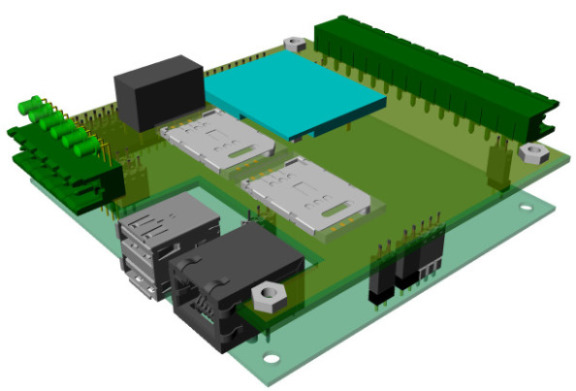
\includegraphics[width=0.24\textwidth]{softron2.jpg}
         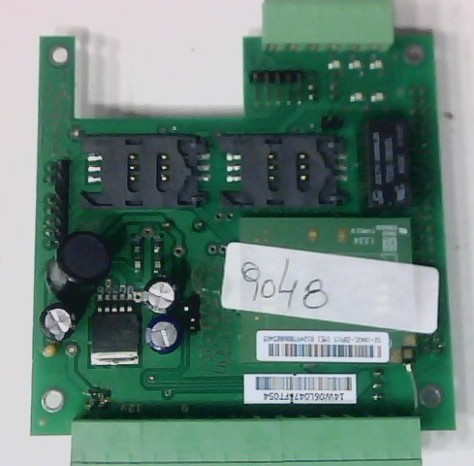
\includegraphics[width=0.24\textwidth]{softron3.jpg}
         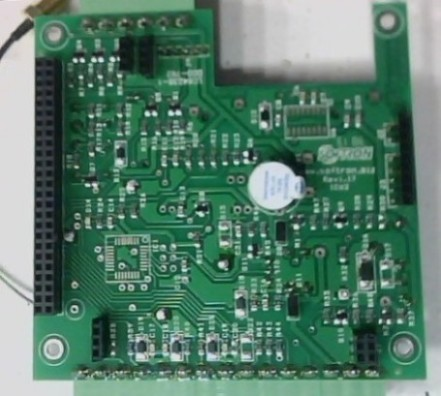
\includegraphics[width=0.24\textwidth]{softron4.jpg}
      \end{center}
      \caption{Placa de integracion entre una SBC y una amplia gama de perifericos, modulo GSM, fuente de alimentacion y conectores.}
      \label{fig:softron1}
   \end{figure}
